\documentclass[12pt]{article}
\usepackage[a4paper]{geometry}
\usepackage[english]{babel}
\usepackage[T1]{fontenc}

\usepackage{hyperref}
\usepackage{graphicx}
\usepackage{float}
\usepackage{epstopdf}
\usepackage{listings}

\usepackage{graphicx}
\graphicspath{{figures/}}

% Packages for building tables and tabulars
\usepackage{array}

\usepackage{proof}
\usepackage{semantic}




%%% BEGIN DOCUMENT
\begin{document}

% BEGIN TITLE PAGE
\thispagestyle{empty}
\begin{center}

\large
UNIVERSITY OF TARTU\\[2mm]
\uppercase{Faculty of Mathematics and Computer Science}\\[2mm]
Institute of Computer Science\\
%Specialty of Computer Science\\[2mm]

%\vspace*{\stretch{5}}
\vspace{25mm}

\Large Stenver Jerkku

\vspace{4mm}

\huge Paralell Wilcoxon Signed-rank tests

%\vspace*{\stretch{7}}
\vspace{20mm}

\Large Bachelor's Thesis (6 ECTS)

\end{center}

\vspace{2mm}

\begin{flushright}
 {
 \setlength{\extrarowheight}{5pt}
 \begin{tabular}{r l}
  \sffamily Supervisor: & \sffamily Sven Laur, PhD
 \end{tabular}
 }
\end{flushright}

%\vspace*{\stretch{3}}
\vspace{10mm}

{\noindent Author: .................................................................................... ``.....'' ..........\hskip16pt 2012}
\vspace{2mm}

{\noindent Supervisor: ............................................................................... ``.....'' ..........\hskip16pt 2012}

\vspace{8mm}

{\noindent Allowed to defence}

{\noindent Professor: ................................................................................. ``.....'' ..........\hskip16pt 2012}

\vfill
\centerline{Tartu 2012}

\newpage

\tableofcontents

\pagebreak

\begin{abstract}
The goal of this project is to create a C++ library that can be run from R statistics program and terminal. The library should be able to run tens of thousands of Wilcoxon Signed Ranked Tests in parallel in mere seconds. It should also be able to run these tests accurately, regardless of the sample size(The number of pairs) and take into account that some test might be missing or flawed. The library is developed for BIIT(Bioinformatics, Algorithmics and Data mining group). BIIT is joint research group between the Department of Computer Science (University of Tartu), Quretec, and the Estonian Biocenter. Its main research topics and capabilities include the gene regulation, gene expression data analysis, biological data mining and others.
\end{abstract}

\newpage

\section{Introduction}
The BIIT research group has biologist who conduct a variety of experiments on a control group. They try to measure, compare and test different attributes of a living organism. These attributes might be, but not limited to blood pressure, proteine amount in the blood, RNA amount, purity of urine, brainwaves etc. These attributes can be repeadedly measured on the same subject and the results are never exactly the same. There is always a little noise and varience between the samples. Biologist often experiment on the control group and try to affect these observed attributes. The take samples before and after simulating the observable attribute with some stimulant. This is called the case-control study.

However, since even without external stimulation the 2 results are never the same. Also, different experiments can have wildly different assumptions, so you cannot simply use a constant error margin on all your tests. For example, the blood pressure measuring before and after jogging could have a lot bigger changes then brainwave changes.  Therefore  the biologist need to use statistical tests to find out which case-control studies are actually significant and which are simply noise.

There are many case-control tests available. For example paired Students t-test, t-test for matched pairs and Wilcoxon signed-rank test. The Wilcoxon signed-rank test is used when the measurement values are not normally distributed when the experimental conditions are fixed.  In practise, this means that the histogram of measurements is either asymmetrical or it does not resemble the bell shape.

It is common to assume that properly scaled gene expression measurements follow normal distribution, while quantities of proteins and metabolites are assumed to have non-normal distribution.

\subsection{NetCDF file format}
The BIIT group holds statistical data in NetCDF file format. NetCDF is an open source standard of a set of data formats, programming interfaces, and software libraries that help read and write scientific data files. \url{http://www.unidata.ucar.edu/software/netcdf/docs/what_is_netcdf.html}$^2$
Data can be held in a structured manner in a NetCDF file. You can define dimensions, name them, put variables in the dimensions and later retrieve or change them. This is useful, for example, to hold matrix like data in a file and have fast lookups. In addition, you can define helper dimensions for the matrix for extra information.
NetCDF file format is used by the BIIT researh group to hold gene data and will be given as an input file for the program.

Currently the BIIT group holds the data in the NetCDF file in the following format:

\textbf{Data matrix}
\begin{itemize}
  \item double data(m, n) - the data matrix of m genes (variables) and n samples (experiments, patients, ...)
  \item string gene[m] - gene IDs
  \item string array[n] - sample IDs
\end{itemize}

\textbf{Non-track metadata}
\begin{itemize}
  \item string __FileFormat - EVDF format identifier string. Current value: "ExpressView 1.1".
  \item string __DatasetType - A string identifying the dataset type. This is used to extract data-specific parameters from a global configuration file. See datatypes.conf (ExpressViewConfigFiles) for allowed values.
  \item string[n] Organism - Organism (per column)
  \item string[n] MetadataOrder - Sometimes metadata (including column tracks) may be in a different order than columns in data. This variable is a permutation of the array variable, specifying the order of column variables. This field is deprecated and all column metadata is expected to be in array order in new datasets.
  \item string InvestigationTitle - short title for the dataset
  \item string ExperimentDescription - long description for the dataset
  \item string DatasetID - Optional Source-specific dataset identifier, e.g. "E-TOXM-3"
  \item string DatasetLink - Optional A URL associated with the dataset, e.g. " http://www.ebi.ac.uk/microarray-as/ae/browse.html?keywords=E-TOXM-3"
  \item string __VariableLabel - Optional Custom variable type name for the dataset (e.g. "probe", "peptide", "sequence"). Overriden by variable_label in project configuration. (ExpressView)
Names of any other (optional, non-track) metadata variables must be prepended by two underscores. Additional variables may be mandated by a data type specification, see ExpressViewConfigFiles. Known specific variables:
  \item string __Organism - ArrayExpress chip organism (ArrayExpress; as opposed to the source of biological material stored in Organism)
\end{itemize}

\textbf{Tracks}

Tracks are all other variables whose name begins with an uppercase character, that are arrays of either string or double, with the size of their first dimension either m or n. The former are referred to asrow tracks and the latter as column tracks. These variables encode some information about either the rows or columns of the data matrix; e.g. ExpressView displays column tracks above the heatmap.

Examples:

string Chemotherapy[n]
string Local\ Relapse[n]
double RelativeVariance[m]

\subsection{Current BIIT procedures}
Currently the BIIT group has 3 ways of analysing its data.
\subsubsection{GNU R}
They can use GNU R project to make custom and complext analyses. For that they need to manually read NetCDF file to the R and then call the R built in function wilcox.test to use Wilcoxon test. The problem with R wilcoxon test is that it is slow. If you run thousands of tests in a row, the results might come after hours of computer processing. One of the goals of this paper and project is to make Wilcoxon test run on command line in mere seconds.
\subsubsection(Web interface)
They can use a web interface which can take in certain arguments and command line script. It then will use whatever command line tools it has available and visualizes the output.

\subsubsubsection(Command line)
They can also use the command line directly which has a variety of tools installed. The wilcoxon test will ultimately call R wilcoxon function.

So in the end - no matter how the biologist analyse their data, they will always use wilcoxon test in the GNU R project.

\subsection{Definitions}

\begin{enumerate}
\item
$N$ - The sample size in a wilcoxon signed-rank test.
\item
$V(N, k)$ - table. We need this table only, for calculating $P(N, k)$. It has no other use for us. It signifies the number of different possible signs in an $N$ sized rank array where $k = W$.  So for example, $V(3, 0)$ would tell us that if we have 3 variables, then how many different signs could those ranks have, if their sum is 0.
\item
$P$ - Value that has been calculated. We need it because we want to know how accurate approximated P value is in practical use, using the V table by using the following formula:
\item
$P = \sum\limits_{k=W}^{\infty} \frac{V(N, k)}{2^n}$
\item
$P(N, k)$ - table that has $P$ values in it for every $N$ and $K$. The table gets exponentially larger, the bigger $N$ is. Table with the size $N=80$ is around 2.5 MB in plaintext file, while $N=800$ is many gigabytes.
\item
$P_{approx}$ - value that has been calculated with the Gaussian Distribution formulae.
\item
$P_{approx}(N, k)$ - table that holds every Papprox value for each $N$ and $K$.
\item
$X$ - the high enough $N$ value where using Gaussian Distribution is accurate enough that we can use, instead of a accurate $P$ table.
\end{enumerate}

\newpage

\section{Wilcoxon signed-rank test}

The Wilcoxon signed-rank test is a non-parametric(data doesnt have to have characteristic parameters or structure) statistical hypothesis test used when comparing two related samples, matched samples, or repeated measurements on a single sample to assess whether their population mean ranks differ - i.e. it is a paired difference test.

This means that with Wilcoxon test you can look at some measurable feature(eg. gene). If we have made two or more experiments in different conditions on it(eg gene experiments and their confirmation results), we can compare them with the test to see if they are relevant. $H_0$ means that the difference between pairs is zero. $H_1$ means it is not.

It was popularized by Sidney Siegel in his book "Nonparametric statistics - for the behavioral sciences". Sidney used the symbol $T$, instead of $W$ in his book, because it was related, but not exactly the same as $W$. Because of this the test is sometimes referred to as the Wilcoxon T test and the test statistic is reported as a value of $T$.

\begin{figure}[!h]
  \centering
  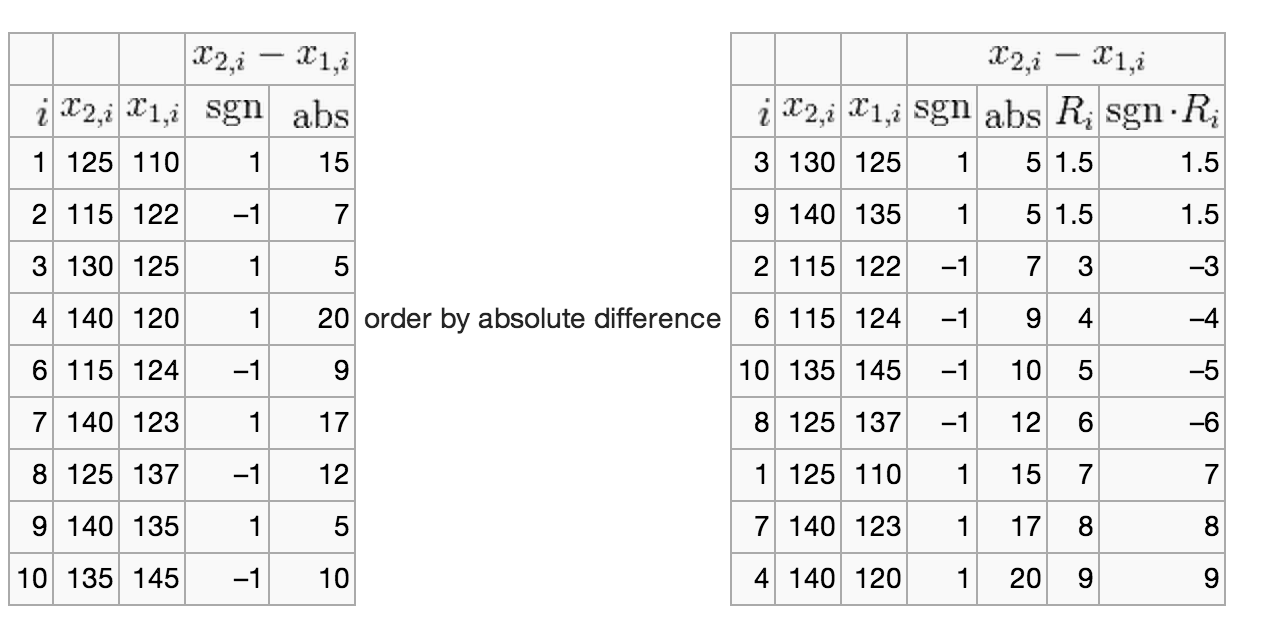
\includegraphics[width=0.8\textwidth]{wilcoxon_test_intro}
  \caption{Wilcoxon test hypothesis table}
  \label{fig:wilcoxon_test_intro}
\end{figure}

\subsection(Statistical Tests)

The statistical tests are usually done, because initial research has raised a hypothesis of which we want to know weather it is true or not.

\begin{figure}[!h]
  \centering
  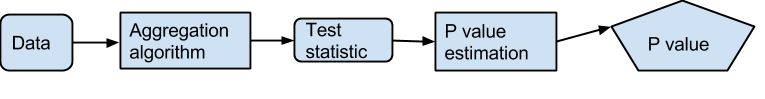
\includegraphics[width=0.8\textwidth]{statisticalTestFlow}
  \caption{Graphical represenation of statistical test flow}
  \label{fig:statisticalTestFlow}
\end{figure}

\subsubsection(Data and aggregation)
Statistical tests are usually built by first gathering the necessary raw data. The data is then organized by some kind of aggregation algorithm which also might filter out tests that dont fall under the assumptions.

\subsubsection(Test Statistic and hypothesis)
Next a test statitic T and hypothesis are stated.

The test statistic is a scalar function of all the observations, which summarizes the data by a single number. Commonly the T is either one-sample, two-sample or paired statistic, depending on the tests. Other statistics might also be used.

The hypothesis raised are null hypothesis and alternative hypothesis. Null hypothesis in a simple terms means false. A more precise explanation would be default position, or that the measured samples have no relationship in between them. It is simple to think of it as a no statement, even though it might not be as accurate. The alternative hypothesis is the opposite - in simple terms, one could think of it as true or interesting result. It means that the two measured samples have a relationship between them, either in direct or indirect ways. A good example to explain these 2 is the court verdict - if null hypothesis is kept, then the suspect has not been found quilty. There was not enough evidence. On the contrary, if null hypothesis was rejected, the suspect was found quilty, because there was enough evidence to make that decision.

When the null hypothesis is true, then the test statistic has a well-defined probability distribution. This means that one can predict pretty well the possible outcome of a measurable subset of samples. The alternative hypothesis sample outcomes are at the edges of a probability distributions, which makes them hard to predict.

\subsubsection(P value estimation)
After that a P value estimation is made with some algorithm. A variety of algorithms have been thought of, depending on the type of data, goals of the tests and even the amount of data. Statistics need to make the right choice between the alorithms by taking all these assumptions into an account. The P value shows the probability that the measured sample belongs in the well-defined probability distribution and where does it most likely belong inside that distribution.

\subsubsection(P value)
Finally a P value is extracted and it can be compared to the critical P value to find out if we should reject or keep the null hypothesis. A certain threshold is taken for the p-value. If the p-value is within this threshold, then null hypothesis is rejected. If the p-value is not within this threshold, then null hypothesis is kept.

Visually, when the probability distribution forms a gaussian distribution, the p-value ranges where the null hypothesis are rejected can be visualized as in ~\ref{fig:p_value_one_sided} and ~\ref{fig:p_value_two_sided}:

\begin{figure}[!h]
  \centering
  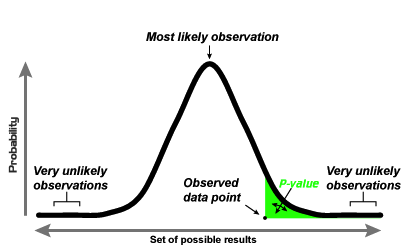
\includegraphics[width=0.8\textwidth]{p_value_one_sided}
  \caption{One sided p value representation}
  \label{fig:p_value_one_sided}
\end{figure}

\begin{figure}[!h]
  \centering
  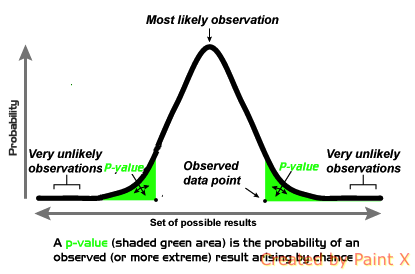
\includegraphics[width=0.8\textwidth]{p_value_two_sided}
  \caption{Two sided p value representation}
  \label{fig:p_value_two_sided}
\end{figure}

\subsection{Wilcoxon test}

\subsubsection{Wilcoxon test Assumptions}
1. Data is from the same population and paired.
2. Pairs are independent and random.
3. The data is measured at least on an ordinal scale - i.e. it allows rank order by which data can be sorted.
4. The median has symmetric distribution of differences.

\subsubsection{Practical use}
Wilcoxon test can be used to make sure that something has an effect on the measured samples. For example, biologist could measure 3 patients white blood cell levels, create some external stimulation on the pations and measure the white blood cell levels again. The wilcoxon signed-ranked test shows wether the external stimulation had any statistical effect on the white blood cell levels.

\begin{figure}[!h]
  \centering
  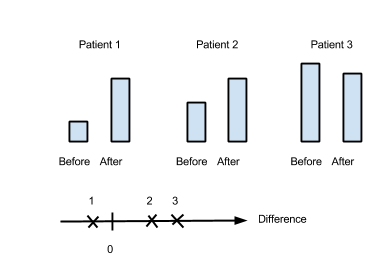
\includegraphics[width=0.8\textwidth]{patientExample}
  \caption{Two sided p value representation}
  \label{fig:patientExample}
\end{figure}

A Test statistic is created for the test that estimates symmetry, but neglets actual value. This means that without the estimation, the statistical analysis of the test would be very difficult, since there is no well-defined probability distribution. However, since the Wilcoxon test estimates symmetry, our probability distribution starts to take the shape of gaussian distribution.

\begin{figure}[!h]
  \centering
  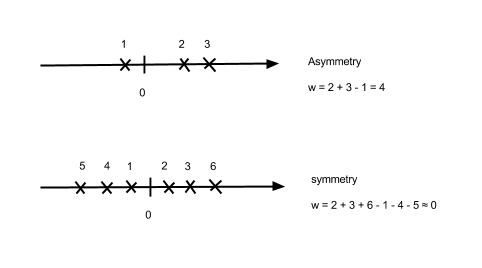
\includegraphics[width=0.8\textwidth]{symmetriassymetry}
  \caption{Two sided p value representation}
  \label{fig:symmetriassymetry}
\end{figure}

\subsubsection{P-value assignement problem}


\subsubsection{The formulae}

The test first ranks the experiment values in an ascending list by subtracting the test experiment value from the original experiment value and then taking absolute value of it. Then it sorts them by size.(pairs $(3, 5), (6, 3), (5, 10)$ would come $-2, 3, -5$, their absolute values would be ranked $1, 2, 3$)

Then it finds out the sign of each experiment pairs(pairs $(3, 5), (6, 3), (5, 10)$ would come $-2, 3, -5$, which signs would be $-, +, -$, in another words, $-1, 1, -1$)

Then it calculates the statistic $W$, which is the absolute value of the sum of the signed ranks, and finds out whether the $N$ is large enough to approximate $P$ value or it needs to use $P$ value table to get the $P$ value. If it can approximate $P$ value, the test calculates $Z$ value and compares it to approximated $Z$ value. If the $Z$ value is bigger than Zcritical, reject $H_0$ . If it cant, then it will just get the $P$ value from built in table and if the $P$ is smaller than $0.05$, then reject $H_0$. The formula for wilcoxon test:

Let $N$ be the sample size, the number of pairs. Thus, there are a total of $2*N$ data points. For $i=1,...,N$, let $x_{1, i}$ and $x_{2, i}$ denote the measurements.

\begin{enumerate}
\item
For $i=1, .., N$, calculate $|x_{2,i} - x_{1,i}|$ and $sgn(x_{2,1} - x_{1,i})$, where  is the sign function.
\item
Order the $N$ pairs from smallest absolute difference to largest absolute difference, $|x_{2,i} - x_{1,i}|$.
\item
Rank the pairs, starting with the smallest as $1$. Ties receive a rank equal to the average of the ranks they span. Let $R_i$ denote the rank.
\item
Calculate the test statistic $W$, the absolute value of the sum of the signed ranks. $W=|\sum\limits_{i=1}^{N} [sgn(x_{2,i} - x_{1,i})*R_i]|$
\item
As $N$ increases, the sampling distribution of $W$ converges to a normal distribution. Where $X$ depends on how accurate you want your results to be
\begin{enumerate}
\item
For $N >= X$, a $z-score$ can be calculated as

$z=\frac{W-0.5}{\sigma_w},\sigma_w = \sqrt{\frac{N(N + 1)(2N + 1)}{6}}$

If $Z > Zcritical$ then reject $H_0$, where $Z_{critical}$ is calculated with Gaussian distribution

\item
For $N < X$, $W$  is compared to a $p-value$ that can be calculated from enumeration of all possible combinations of $W$ given $N$.

If $W >= P_{critical}$, $N$ then reject $H_0$
\end{enumerate}
\end{enumerate}

\subsubsection{Example}
Given pairs $[{6, 8}, {3, 3}, {2, -3}, {-3, 3}, {1, 3}]$.

1. Calculate absolute values and signs:
Absolute values $[2, 0, -5, 6, 2]$
Signs $[1, 0, -1, 1, 1]$
2. Exclude pairs absolute value is $0$
3. Order the remaining pairs. Ties receive therank equal to average of the ranks they span
$[{2 => 2.5}, {-5 => 1}, {6 => 4}, {2 => 2.5}]$
4. Calculate the test statistic W
$W = 1*2.5 + (-1*1) + 1*4 + 1*2.5$ = 8
5. Since $N_r$ is very small, we use a table to look up the $p$ value. The calculation of $p$ table is in a later chapter.
$P(5, 8) = 0.125$
Since $0.125 > 0.05$, reject $H_0$

\subsection{Bonferroni correction}

If you make multiple hypothesis on a test, then you increase the risk in which you reject null hypotheses when its actually true. The Bonferroni test helps to counteract this in a simple way - for each hypothesis you make on a test, you should use a significance level $N$ times lower than before. So for example, if you make $N$ hypothesis and want want a significance level $α$,  then you should run each test at a significance level of $α/N$.

If you want to use Bonferron correction with Wilcoxon signed-rank test, then you need to keep in mind that the approximated $P$ value significance level needs to be much more accurate, since the bonferron test divides it by the amount of features tested. This means higher the $X$ value, the more features you add in the test. \url{http://en.wikipedia.org/wiki/Bonferroni_correction}$^3$

\subsection{Calculating Exact P table}
\subsubsection{Theory}
The P exact table is calculated by counting the number of different ways one can add or substract ranks with each other so he gets a certain sum.

For example, when $N$ is $3$, given ${0, 1, 2}$, one can combine them into $0 + 1 + 2$ or $0 + 1 - 2$ or $0 - 1 + 2$ or $0 - 1 - 2$. This gives us one way to get $3$, one way to get $1$, one way to get $-1$ and one way to get $-3$

This counting of possibilities can be continued until infinity and it forms a normal distribution that widens very fast. The edge of the distribution on a certain $N$ is equal to the sum of every value until $N$

Once the distribution with large enough $N$ is calculated, you can calculate the probability $P$ that a combination of ranks falls into that sum. In other words given distribution table $V$ which shows how many different possibilities there is to combine ranks to get a certain sum given a certain number of ranks, we can calculate the probability that our ranks form that certain sum.

For example, when $N$ is $3$, given $0, 1, 2$, we can calculate that the probability that our there is a $0.25\%$ that our value is $3$ or lower and $0.5\%$ that our value is $1$ or lower.

This distribution is the most accurate table you can compare your wilcoxon test results on - it shows the exact probability that your tests falls into a certain normal distribution range. However, the table is expensive to calculate with $O(n^2)$ complexity.

\subsubsection{The V table formula}
Given $N$ which shows us the number of ranks starting from $0$ and $k$ which shows us the sum that we are interested in. Recursively apply this algorithm until you reach to the $N = 1$.
$V(N+1, k) = V(N, k-1) + V(N, k+N+1)$

There are some additional conditions to the formula:

$V(N, k) = 0$ if $k < -N * \frac{N+1}{2}$ or $k > N * \frac{N+1}{2}$

$V(N, k) = 1$ if $k = -N * \frac{N+1}{2}$ or $k = N * \frac{N+1}{2}$

\subsubsection{The P table formula}
Given $V$ table, $N$ and $k$, we can calculate the $P$ by
$W=|\sum\limits_{T = k}^{\infty}[\frac{V(N, T)}{2^n}]$

To get the P table, we go through all $N$ and $K$ values that we are interested in.

\subsubsection{Code sample}
You can find a python implementation of a code sample in
\url{https://bitbucket.org/stenver/wilxoni-astaku-test/src/870cc6112d0de4483cd99c71e651c2d06feaaee9/WilcoxonVTable/WilcoxonVTable.py?at=default}

The $V$ table calculation is showcased in the methods $V$ and $calculateVvalues$

The $P$ table calculation is showcased in the method $calculatePValues$

\newpage

\section{Approximating the P value}

\subsection{Theory}
The biggest problem when calculating $P$ values in the other Wilcoxon signed-rank tests is that when they have the samples $Z$ value, then they need to compare it to a $Z_{critical}$ value. If the number of samples $N$ is sufficiently large, the solution is simple - use the Gaussian Distribution formulas to find the $Z_{critical}$. In the BIIT research group, however, the $N$ is usually not sufficiently large.
However, once the $N$ gets too small, you cant use the Gaussian Distribution anymore. Furthermore, it is not known where exactly the $N$ limit is, so an arbitrary number is used for that purpose. The currently suggested $N$ is 10.$^4$
In the case the $N$ gets too small, you cant use $Z$. You must instead use $W$ and you can calculate the $W_{critical}$ by
Calculating the $V(N, k)$ table
Calculate the $W_{critical}$ where $W_{critical} = P(N, k)$:

The bottlenecks here are the two steps . Other implementations of the test calculate the tables every time the test is run, thus if you run thousands of tests in a row, a lot of complex recomputation is done. This eventually becomes a performance issue.
To speed this up - this project will calculate the entire $P(N, k)$ for every value that is possible where $N < X$. Then the $P(N, k)$ will be hardcoded inside the program for quick lookup of the value.
This paper will focus on finding the $X$ value

\newpage

\section{Finding the $X$ value}
\subsection{Proving that $P$ and $P_{approx}$ get more similar as $N$ increases}
First we wanted to confirm that as $N$ grows, $P$ and $P_{approx}$ value will get more and more similar. To do this, we took $P(N, k)$ value for each $N$ where
$N < 50$ and $P(N, k)  = 0$ and $P(N, k - 1) != 0$.
We then compared the $P(N, k)$ and $P_{approx} (N, k)$ for each $N$ where:
The results are on Figure ~\ref{fig:T0vsN}.


\begin{figure}[!h]
	\centering
  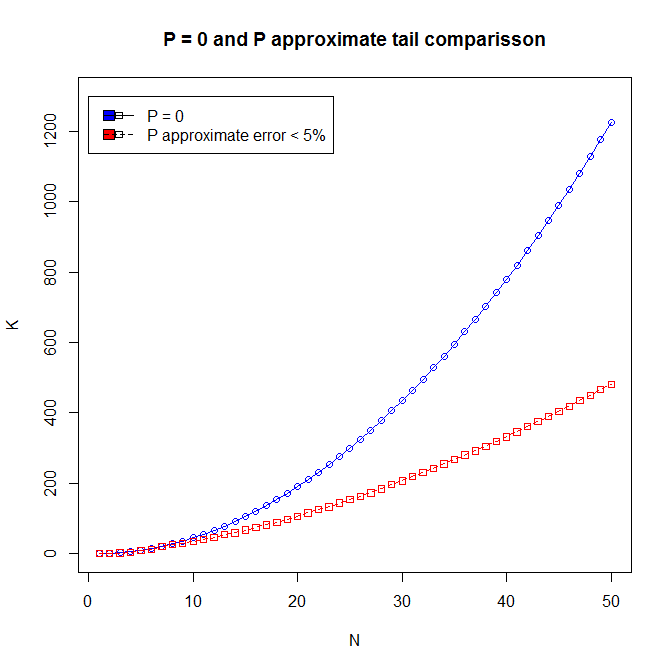
\includegraphics[width=0.8\textwidth]{T0vsN}
	\caption{Approximate and accurate comparisson}
	\label{fig:T0vsN}
\end{figure}

\begin{figure}[!h]
	\centering
  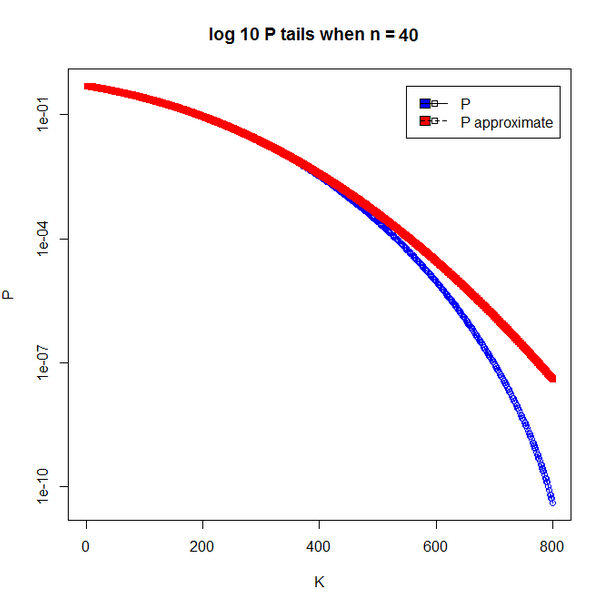
\includegraphics[width=0.8\textwidth]{log10PtailsN40}
	\caption{Relative error increasing toward edge of tail}
	\label{fig:log10PtailsN40}
\end{figure}

Much to our surprise, as $N$ grew, the gap between approximate and accurate $P$ values grew bigger. This meant that as $N$ grows, the Gaussian distribution will get more inaccurate toward the tails of the distribution. Previously we thought that with the growth of $N$, Gaussian would surely get more and more accurate.
From Figure ~\ref{fig:log10PtailsN40} we can see that Gaussian distribution is a little bit bigger and gets bigger as $K$ grows. Figure 2 illustrates the difference in position of between last accurate $P_{appox}$ and $P = 0$. Accurate means that the relvative error is under $5\%$

To further investigate this finding, we decided to find out the minimum $P$ value that you can get for each $N$ while maintaining a certain error threshold. The thresholds chosen were $5\%, 10\%, 20\%, 50\%$. The formula used was the same as before, except the thresholds were replaced as needed.

\begin{figure}[!h]
	\centering
  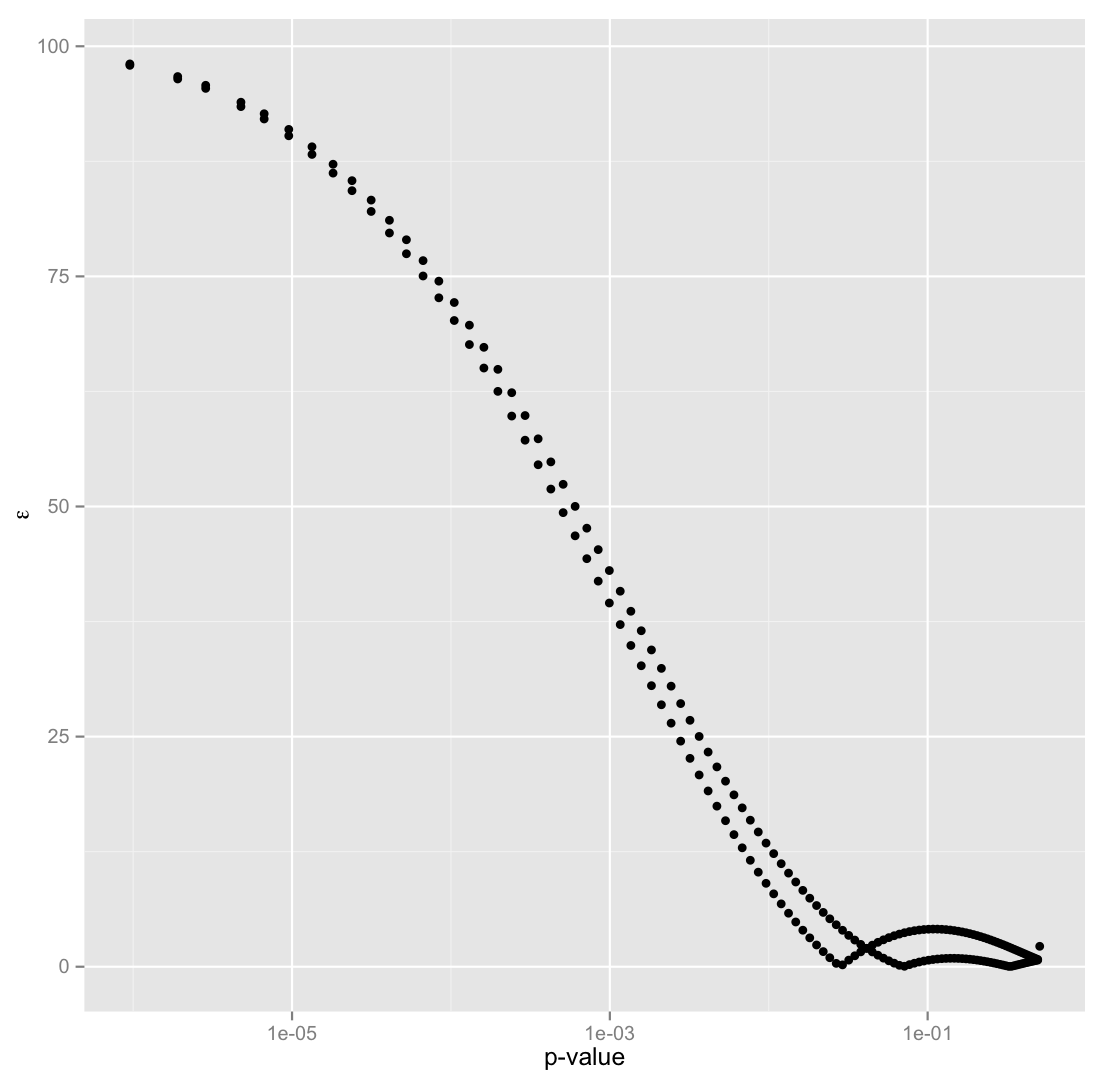
\includegraphics[width=0.8\textwidth]{RelativeErrorDecreasingPgrowsN20}
	\caption{Comparing approximate probability relative error as sample size increses}
	\label{fig:PvsN}
\end{figure}

\begin{figure}[!h]
	\centering
  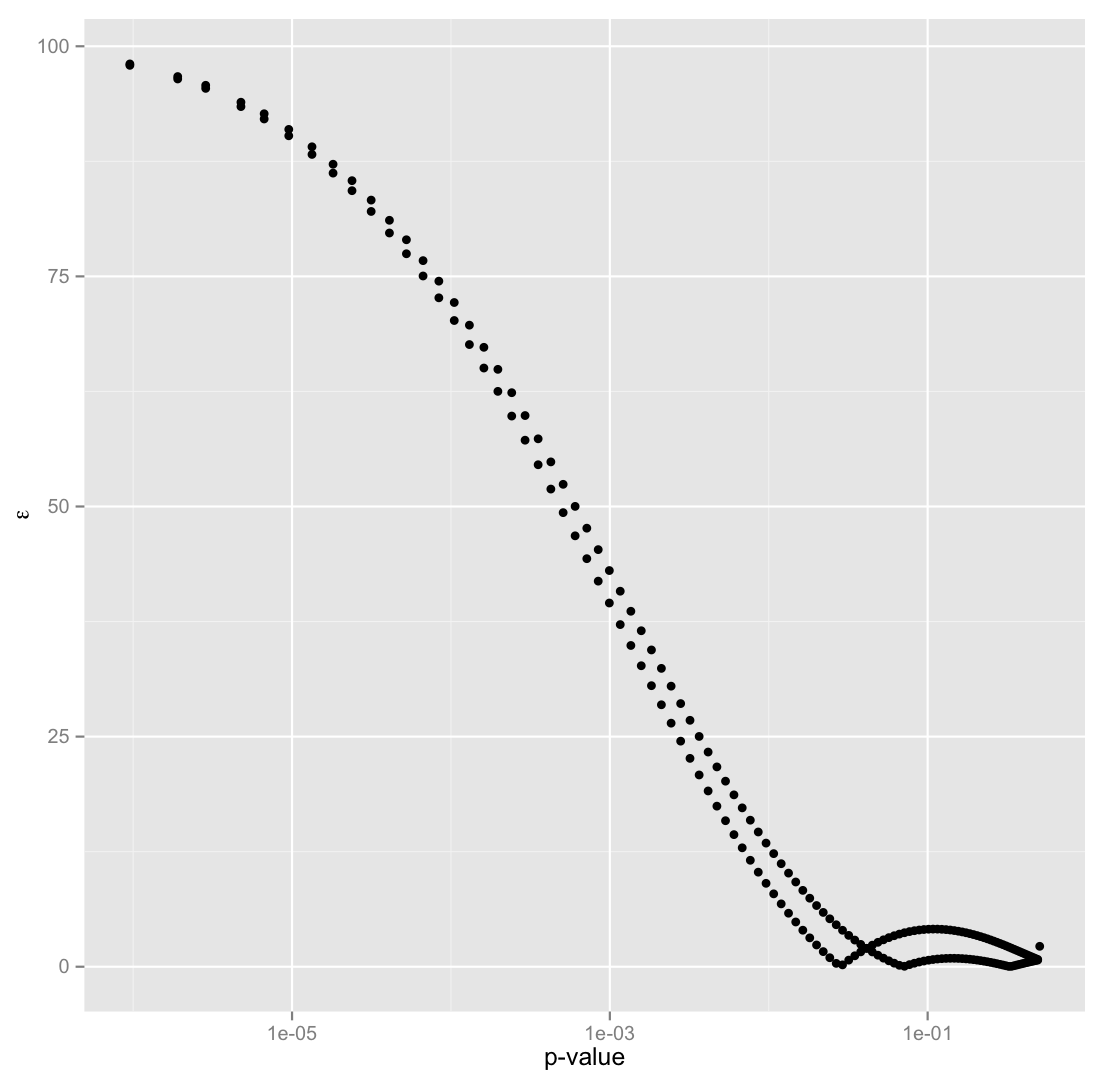
\includegraphics[width=0.8\textwidth]{RelativeErrorDecreasingPgrowsN20}
	\caption{Showing the relative error as probabilty increases when sample size is 20}
	\label{fig:RelativeErrorDecresingPgrows}
\end{figure}

From figure ~\ref{fig:PvsN} we can see that as the $N$ grows, the graph becomes stable, meaning that the distribution becomes a normal distribution at around $N > 10$ and $N < 25$. We can see that the minimum $P$ value under error threshold does get smaller, as $N$ increases, so this further proves that Gaussian distribution does get more accurate as $N$ grows. This is because as $N$ increases, you can take a $P$ value closer to the tail of the distribution and still get an accurate value.

The figure ~\ref{fig:RelativeErrorDecresingPgrows} shows us the relative error as $P$ grows when $N = 20$. The $P$ values are logged on this graph. There are 2 noteworthy things here, however. First, around $P = 0.05$, the relative error actually get a little small tip toward accuracy. Second, it can be seen that there are two accuracy paths that the error takes, depending on weather in $P_{approx}(N, k)$  the $K$ is even or odd number. This is a computational artefact caused by the recurrence of the $V(N, K)$ values and we will not make any conclusions of that.

\subsection{Investigating the $P(N, k)$ and $P_{approx}(N, k)$ similarities}
To further prove that we can start using Gaussian Distribution at a certain $N$, we needed to prove that Papprox will get more accurate as the N increases toward the tail of the distribution aswell.

To achive this, we found out the largest relative error between $P$ and $P_{approx}$ for each $N$ and for each $P$ where $P = (0.5:0.1), P = (0.1, 0.01), P = (0.001, 0.0001), ... , P = (10-14 , 10-15)$

\begin{figure*}
	\centering
  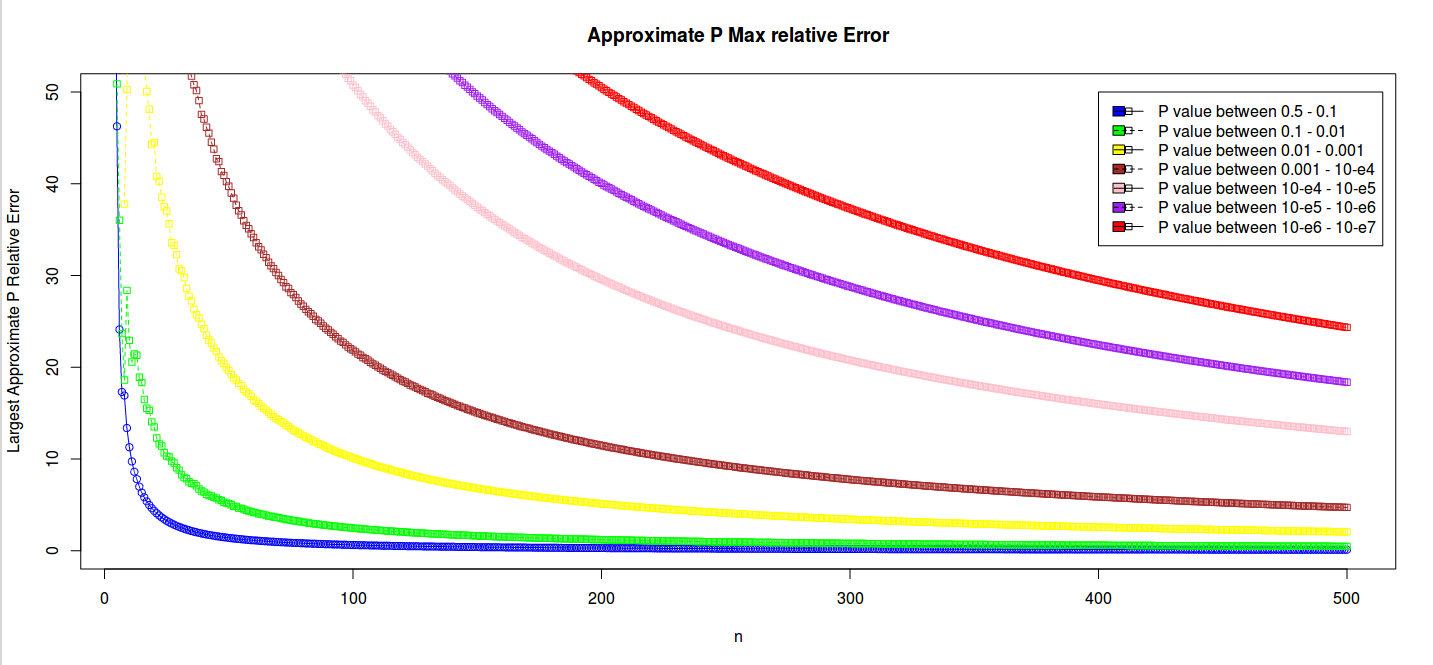
\includegraphics[width=0.8\textwidth]{LargestApproxPRelativeError3}
	\caption{Showing the maximum approximate relative error in probability ranges, as sample size increases}
	\label{fig:LargestApproxPRelativeError}
\end{figure*}

As can be seen from figure ~\ref{fig:LargestApproxPRelativeError}, the relative error increases exponentially. When $P = (10-5 , 10-6)$ the relative error is massive. When $N=200$, then the error is still around $40\%$. The bigger the $N$ gets, the bigger the error at the tail. However, it can also be seen that the error decreases steadily as $N$ grows for each of the $P$ range chosen.

This means that even though the error of the distribution tail edge does increase as N grows, overall, both distributions get more and more similar to the gaussian distribution

To further investigate the relation between $P(N, k)$ and $P_{approx}(N, k)$, we wanted to see the difference between all $P$ values when $P = 50$ and when $P = 25$

\begin{figure}[!h]
	\centering
  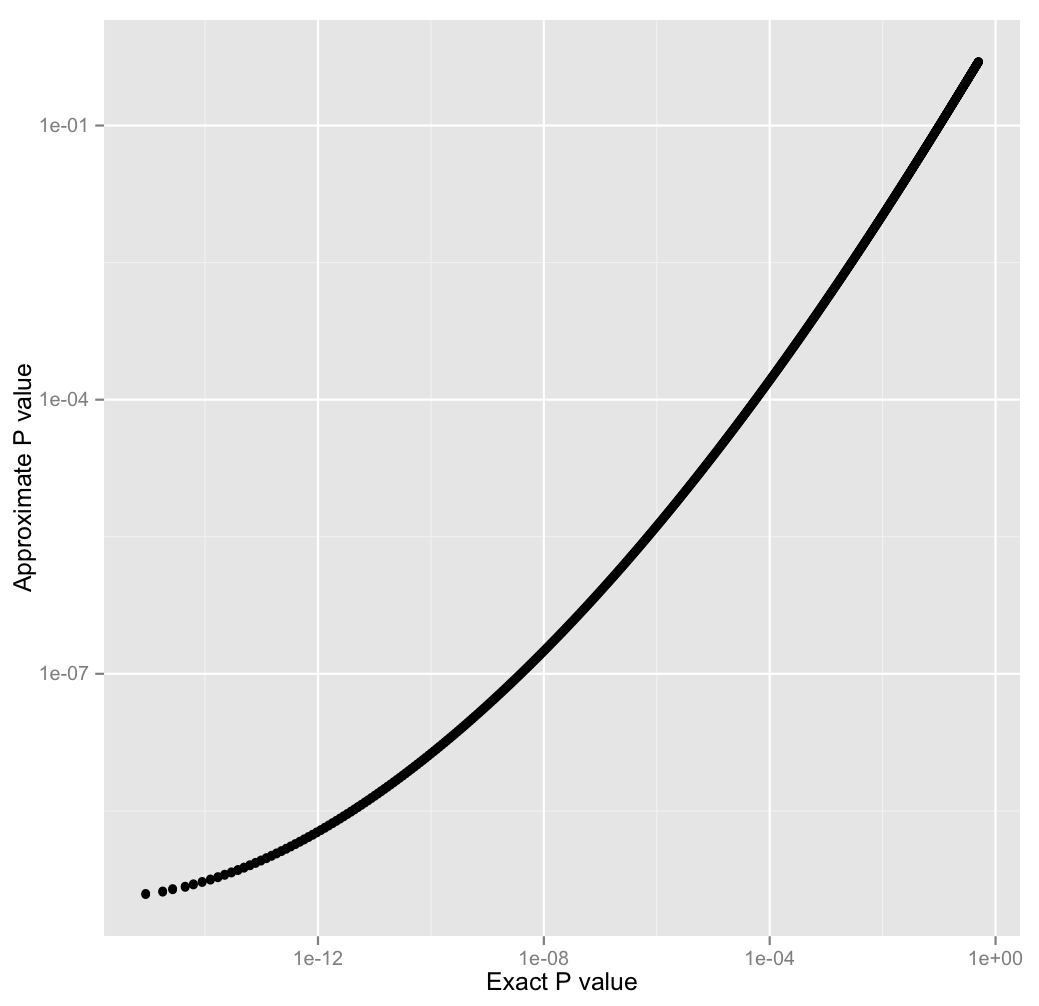
\includegraphics[width=0.8\textwidth]{PvsP50}
	\caption{Relative value of all actual probabilities and approximated probabilities when sample size is 50}
	\label{fig:PvsP50}
\end{figure}

\begin{figure}[!h]
	\centering
  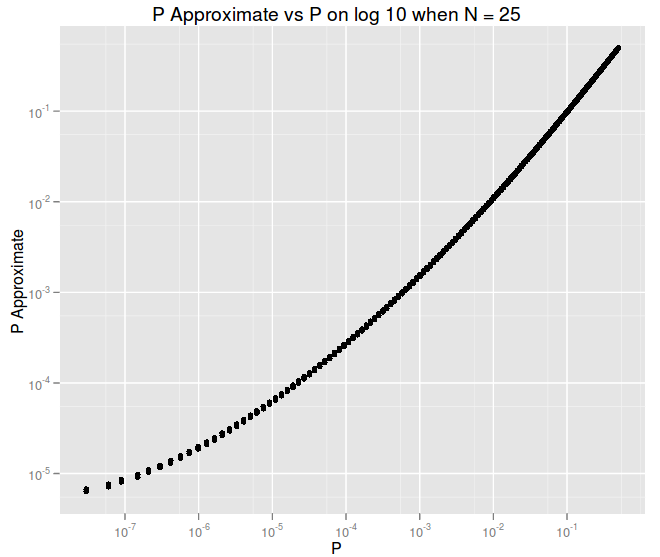
\includegraphics[width=0.8\textwidth]{PvsP25}
	\caption{Relative value of all actual probabilities and approximated probabilities when sample size is 25}
	\label{fig:PvsP25}
\end{figure}

As we can see from ~\ref{fig:PvsP50} or ~\ref{fig:PvsP25}, when the $N = 50$ or $N = 25$, then the $P(N, k)$ and $P_{approx}(N, k)$ values are almost the same with slight differences - the $P_{approximate}$ is a little bit larger. When $N = 25$, the graph is a little less smooth, which tells us that the differences are not as similar as they are when $N = 50$.

\subsection{Determining the X value}
Judging by all the data we have gathered, we can clearly see that as $N$ grows,  $P(N, k)$ and $P_{approx}(N, k)$ tail edges grow apart but overall the distribution gets more and more similar. Determining the $X$ value depends on the amount of data we have and the accuracy of the result we want. The most helpful graphs to help us determine the necessary $X$ value is figure ~\ref{fig:LargestApproxPRelativeError}. Table ~\ref{table:requiredN} illustrates the number of samples($N$) needed for a certain relative accuaracy. So the $X$ value depends on the number of measurements and the required accuracy where $X = N$:

\begin{table}[!h]
	\begin{center}
		\caption{Showing the minimal required sample size for a certain relative error and number of measurements}
	    \begin{tabular}{| l | l | l |}
	    \hline
		Measurements & Error & Required N \\
		\hline
		10 & 5\% & 25 \\
		100 & & 250 \\
		1000 & & 500 \\
		10000 & & $>500$ \\
		100000 & & $> 500$ \\
		\hline
		10  & 10\% & 80 \\
		100 & & 200 \\
		1000 & & $>500$ \\
		10000 & & $>500$ \\
		100000  & & $>500$ \\
		\hline
		10  & 20\% & 50 \\
		100 & & 100 \\
		1000  & & 280 \\
		10000  & & 500 \\
		100000  & & $>500$ \\
		\hline
		10  & 50\% &  25 \\
		100 & & 50 \\
		1000 & & 100 \\
		10000 & & 150 \\
		100000 & & 200 \\
		\hline
		\end{tabular}
		\label{table:requiredN}
	\end{center}
\end{table}
Table \ref{table:requiredN} showing the required N for measurements size while maintaining a relative error

As pointed out in the beginning, when the $N$ grows, the $P(N, k)$ table size grows exponentially. As such, we needed to find a balance between accuaracy and precalculated table thats still within acceptable size.

We chose the size to be $N=80$, since the plaintext file of the precalculated table with that $N$ is around 2.5 MB.

This will allow us to run tests on 10 experiments while maintaining a 10\% accuracy.

Future research could look into approximating the accurate $P(N, k)$ table and potentially decrease the size of the file, increase the precalculated table size while keeping the accuracy relatevly the same.

\newpage

\section{The implementaion}
Repository that contains everything about our findings can be found in

\url{https://bitbucket.org/stenver/wilxoni-astaku-test/src/870cc6112d0d?at=default} repository

The repository contains a number of folders.

\subsection{RcppWilcoxonTest}
 An interface that connects our implementation of the optimized Wilcoxon algorithm to the R. Note that you must have installed our implementation to use it. The interface must be compiled with separate R commands from the command line. You need Rcpp packages for R to use it. It can be installed in R console by running:

\begin{lstlisting}
$install.packages("Rcpp")
\end{lstlisting}

After that, the package can be installed to R by running the command in the command line in the folder:

\begin{lstlisting}
$R CMD INSTALL .
\end{lstlisting}

You can now load our library in R by calling the

\begin{lstlisting}
>library('RcppWilcoxonTest')
\end{lstlisting}

and you invoke the function by calling

\begin{lstlisting}
>RcppWilcoxonTest::WilxTest(dataMatrix,
dataXsize, dataYsize, testIndexes, controlIndexes)
\end{lstlisting}

\subsection{TerminalWilcoxonTest}

An interface that connects our implementation of the optimized Wilcoxon algorithm to the R. Note that you must have installed our implementation to use it. The interface can be compiled by going to the folder, compiling and running help for further help.

\begin{lstlisting}
$make
WilcoxonTest --help
\end{lstlisting}

Currently only supports NetCDF file as input data.

\subsection{WilcoxonTestLibrary}
Our implementation for the optimized wilcoxon test. You library can be installed by going to the folder and running

\begin{lstlisting}
make install
\end{lstlisting}

\subsection{WilcoxonVTable}
Python program that can calculate $V$ and $P$ tables, print them, create files of the tables and create a number of graphs on the tables.

\subsection{Seminar\_paper}
The folder that contains this paper and all images attached to it. It also contains R programs to create those images.

\newpage

\section{Conclusion}
We found out that Gaussian distribution tail edge grows larger apart from the $P(N, K)$ as $N$ increases while the overall distribution grows more similar. In addition, we confirmed that if we want to run thousands of parallel tests, then using approximation is not reliable and instead an accurate table of P values must be used. Calculating that table is very expensive and thus it is advised to precalculate the table for the program. However, our research shows that if we want to have 10 000 measurements run under 5\% relative error, then the hardcoded $N$ should be over 1000. Table of that size would take many gigabytes of space and is impractical to use. For the time being, we will keep the precalculated table $N=80$. This will allow us to make 10 parallel measurements with 10\% error. In the future, we will look into optimizing the precalculated table to use larger data $N$ sizes.

Overall the research included some surprising results and can be considered a success. The library is at its final stages of development and already shows positive results.

\newpage

\section{References}
\begin{enumerate}
\item
[1] Wikipedia Foundation Inc, Wilcoxon Signed-rank test (\url{http://en.wikipedia.org/wiki/Wilcoxon_signed-rank_test}),  14 August 2013
\item
[2] The Unidata Program Center, NetCdf (\url{http://www.unidata.ucar.edu/software/netcdf/docs/what_is_netcdf.html}), 25 September 2013
\item
[3] Wikipedia Foundation Inc, Bonferroni correction (\url{http://en.wikipedia.org/wiki/Bonferroni_correction}), 18 September 2013
\item
[4]  Lowry, Richard. "Concepts \& Applications of Inferential Statistics". (\url{http://vassarstats.net/textbook/ch12a.html}), 24 March 2011.
\end{enumerate}

\end{document}
